The full differential cross section for this process can be expressed by \eqref{eq:DVPiPCrossSection_theory}

        \begin{equation*}
          \recallLabel{eq:DVPiPCrossSection_theory}.
        \end{equation*}

In practice, it is easier to work with the reduced form of the cross section with the virtual photon flux factor $\Gamma$ factored out, as given by \eqref{eq:xsec_reduced}.

 \begin{equation}\label{eq:xsec_reduced}
    \frac{d^2\sigma_{\gamma^*p \rightarrow p'\pi^0}(Q^2,x_B,t,\phi_{\pi},E)}{dtd\phi} = \frac{1}{\Gamma_V(Q^2,x_B,E)} \frac{d^4\sigma_{\gamma^*p \rightarrow p'\pi^0}}{dQ^2dx_Bdtd\phi_{\pi}}.
\end{equation}

The results of this work are presented as reduced cross sections in the following pages. There were 1841 total 4-fold differential bins that passed all selection criteria. Example results are shown for sample bins in \figref{fig:redxsec_phi}. Data points are black points with error bars (black=statistical only, red = total). The black curve is a A+B$\cos(\phi)$ +C$\cos(2\phi)$ fit to the data to allow for structure extraction, the results of which are discussed in Chapter \ref{Chapter:Further Analysis}. The blue curve is the result from the CLAS6 experiment \parencite{Bedlinskiy2014ExclusiveCLAS} adjusted for the difference in beam energy. The blue band surrounding the blue curve is the approximate error for the CLAS6 result.


\iffalse
 \begin{equation}\label{xsec_red_full}
    \frac{d^2\sigma_{\gamma^*p \rightarrow p'\pi^0}}{dtd\phi} = \frac{1}{\Gamma_V(Q^2,x_B,E)} \frac{N(Q^2,x_B,t,\phi_{\pi})}{\Lumi_{int}\Delta Q^2\Delta x_B\Delta t\Delta \phi} \frac{1}{\epsilon_{ACC} \delta_{RC} \delta_{Norm} Br(\pi^0 \rightarrow \gamma \gamma)}
\end{equation}

\fi

\begin{figure}[H]
    \centering

    \subfloat[$\langle x_B \rangle$=0.23,$\langle Q^2 \rangle$=1.73 $GeV^2$,$\langle t \rangle$=0.26 $GeV^2$]{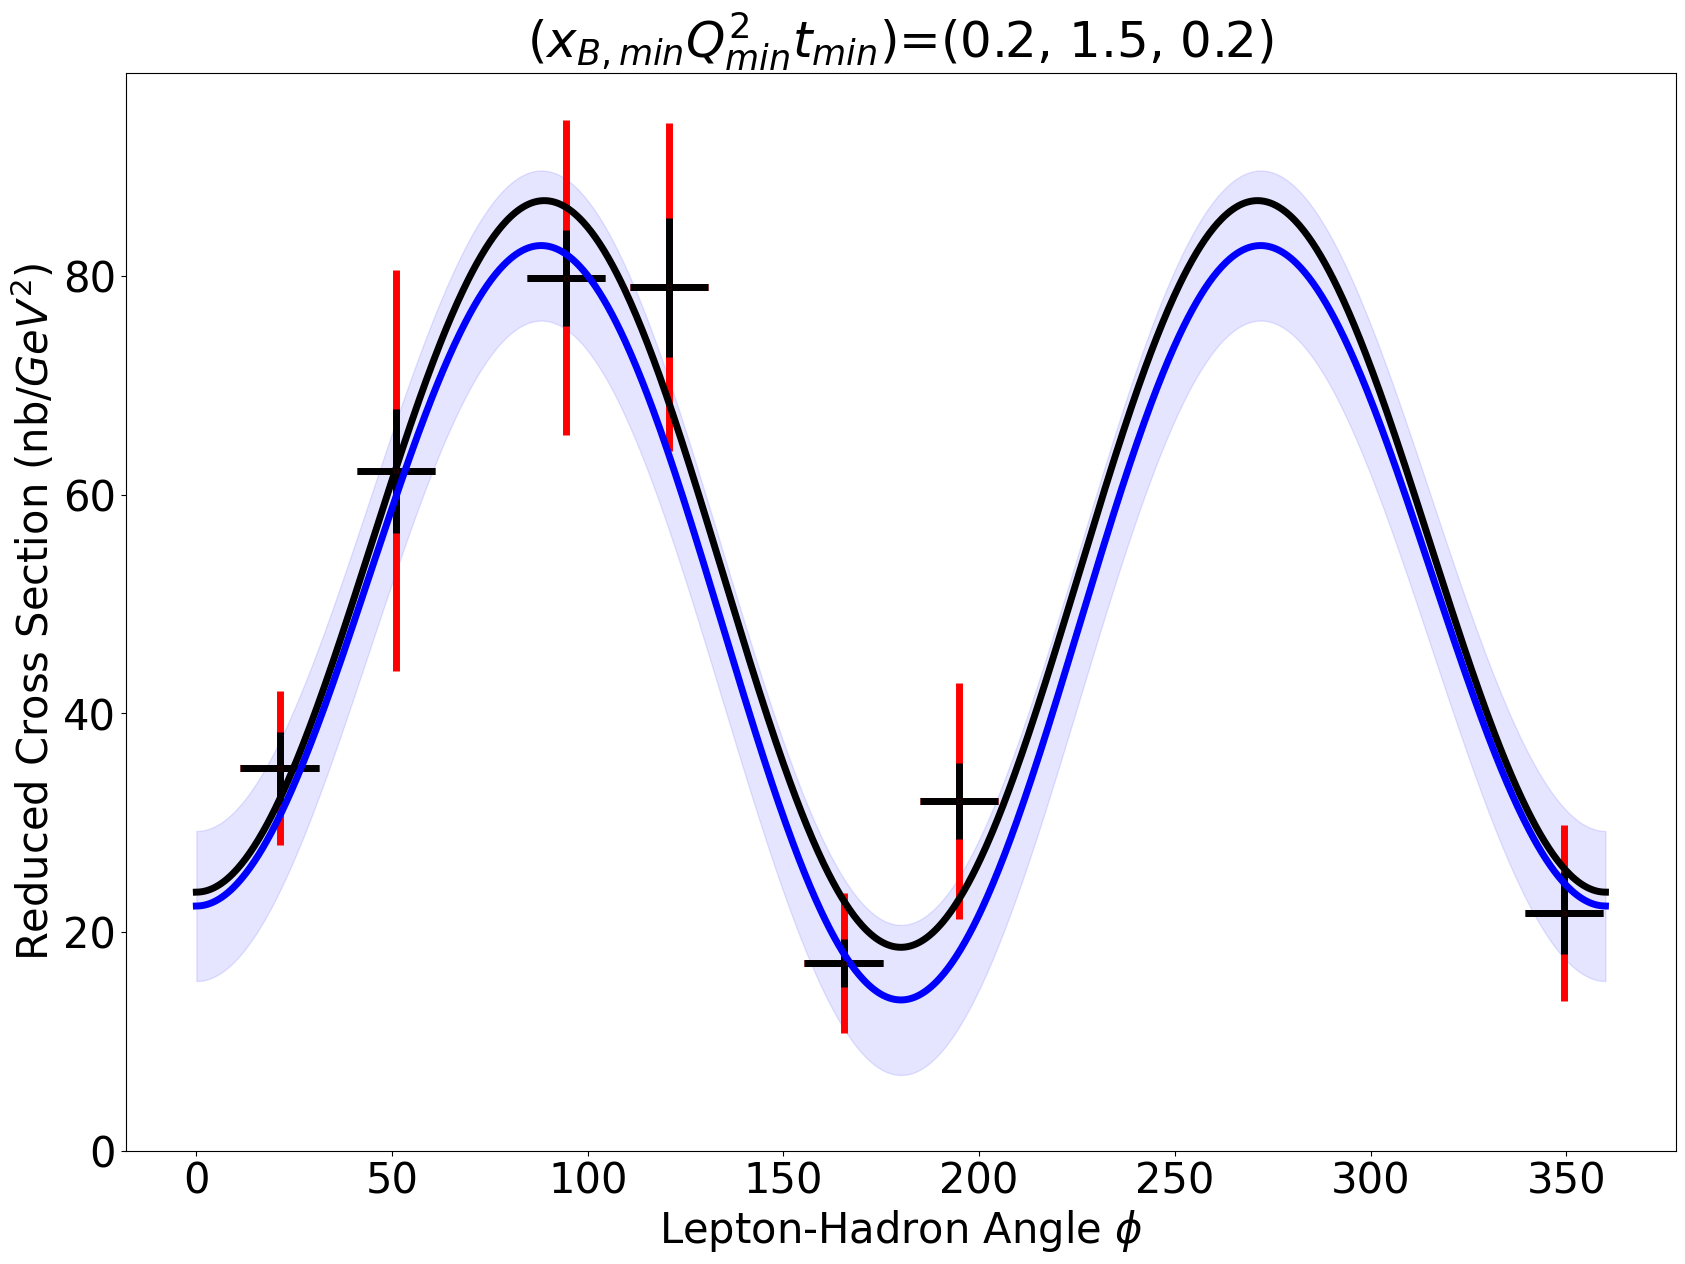
\includegraphics[width=0.5\textwidth]{Chapters/Ch4-BaseAnalysis/bin_by_bin_cross_sections/singles/xqt=(0.2, 1.5, 0.2).png}}
    \hfill
    \subfloat[$\langle x_B \rangle$=0.62,$\langle Q^2 \rangle$=7.88 $GeV^2$,$\langle t \rangle$=1.24 $GeV^2$]{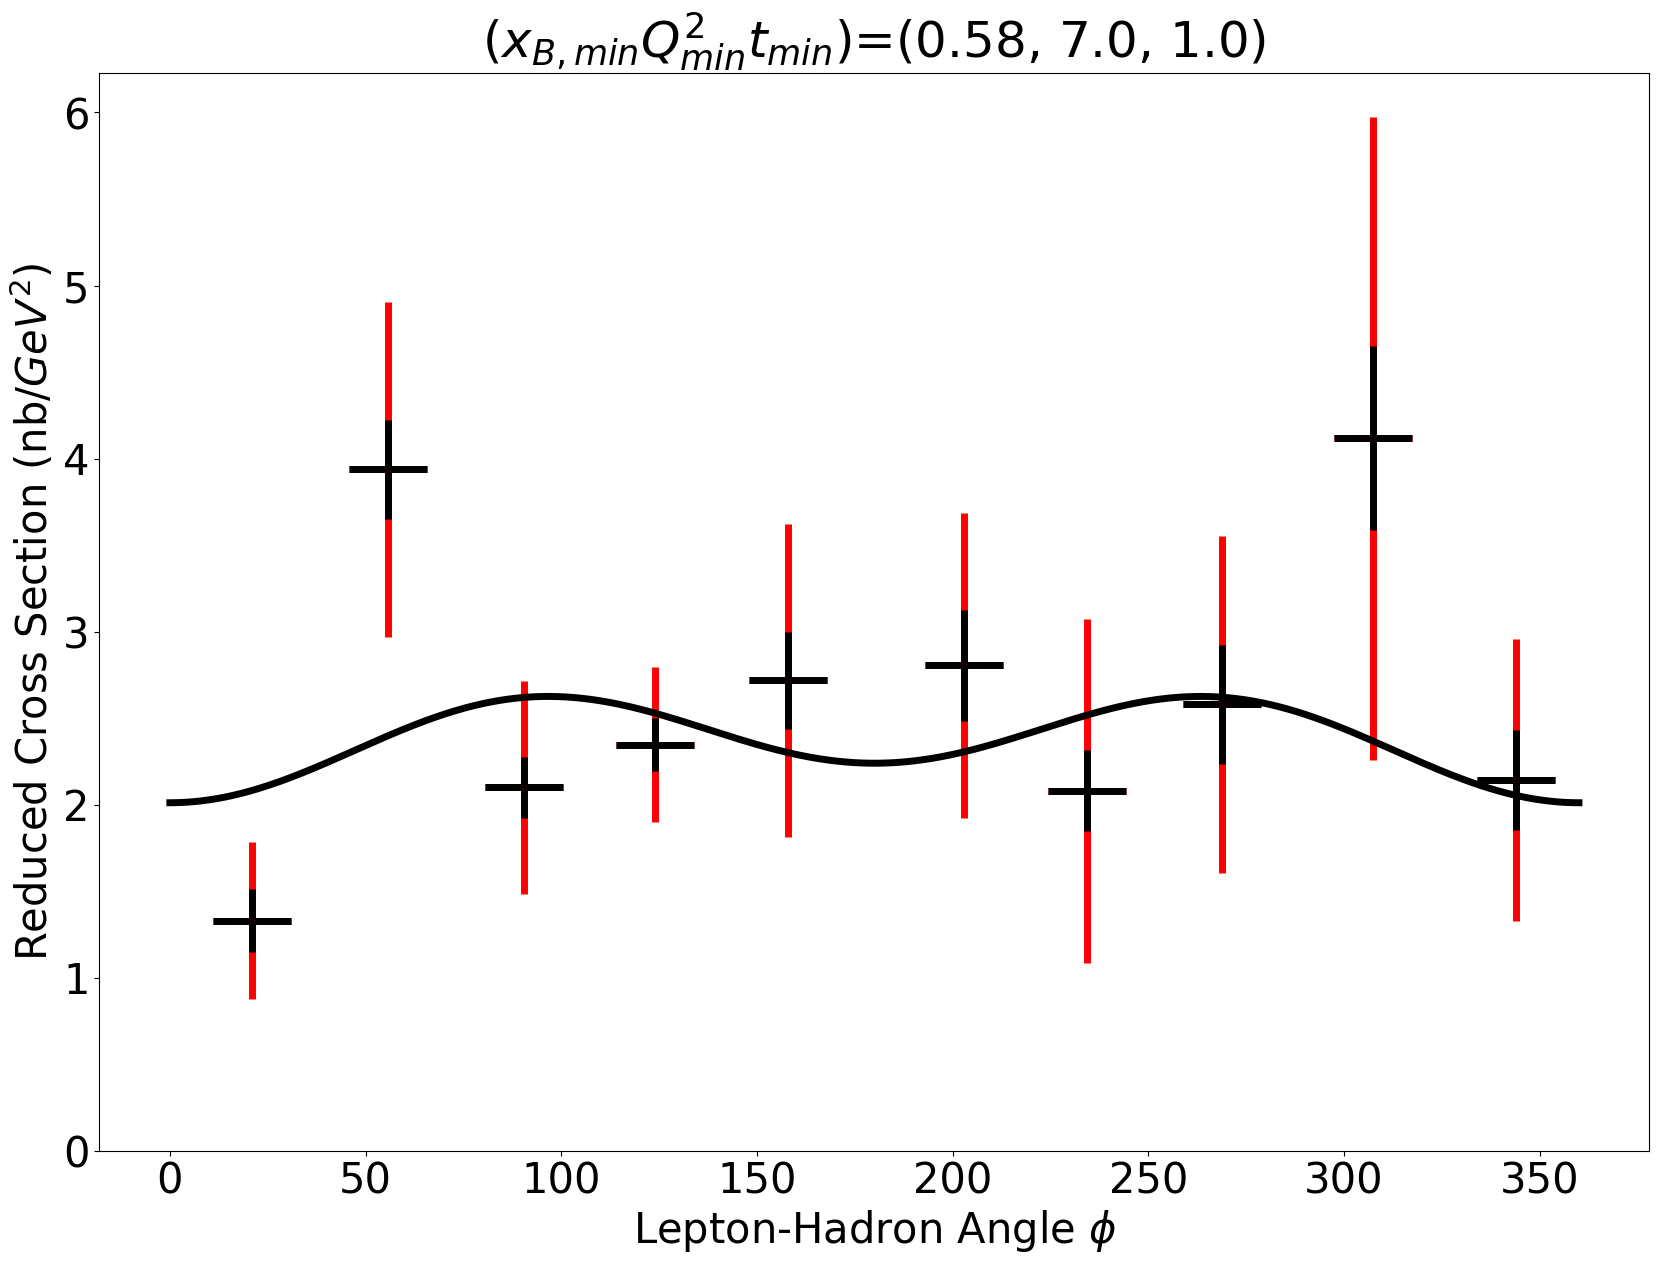
\includegraphics[width=0.5\textwidth]{Chapters/Ch4-BaseAnalysis/bin_by_bin_cross_sections/singles/xqt=(0.58, 7.0, 1.0).png}}

    \caption[Reduced Cross Sections Across $\phi$]{Reduced cross sections across $\phi$ at (a) low kinematics and (b) high kinematics. Where kinematic overlap exists, the CLAS6 result \parencite{Bedlinskiy2014ExclusiveCLAS} is shown in blue with an error band (in modified form to account for beam energy differences). }\label{fig:redxsec_phi}
    %\caption[Reduced Cross Sections Across $\phi$]{Reduced Cross Sections Across $\phi$}
\end{figure}




\iffalse

\begin{figure}[ht]
\centering
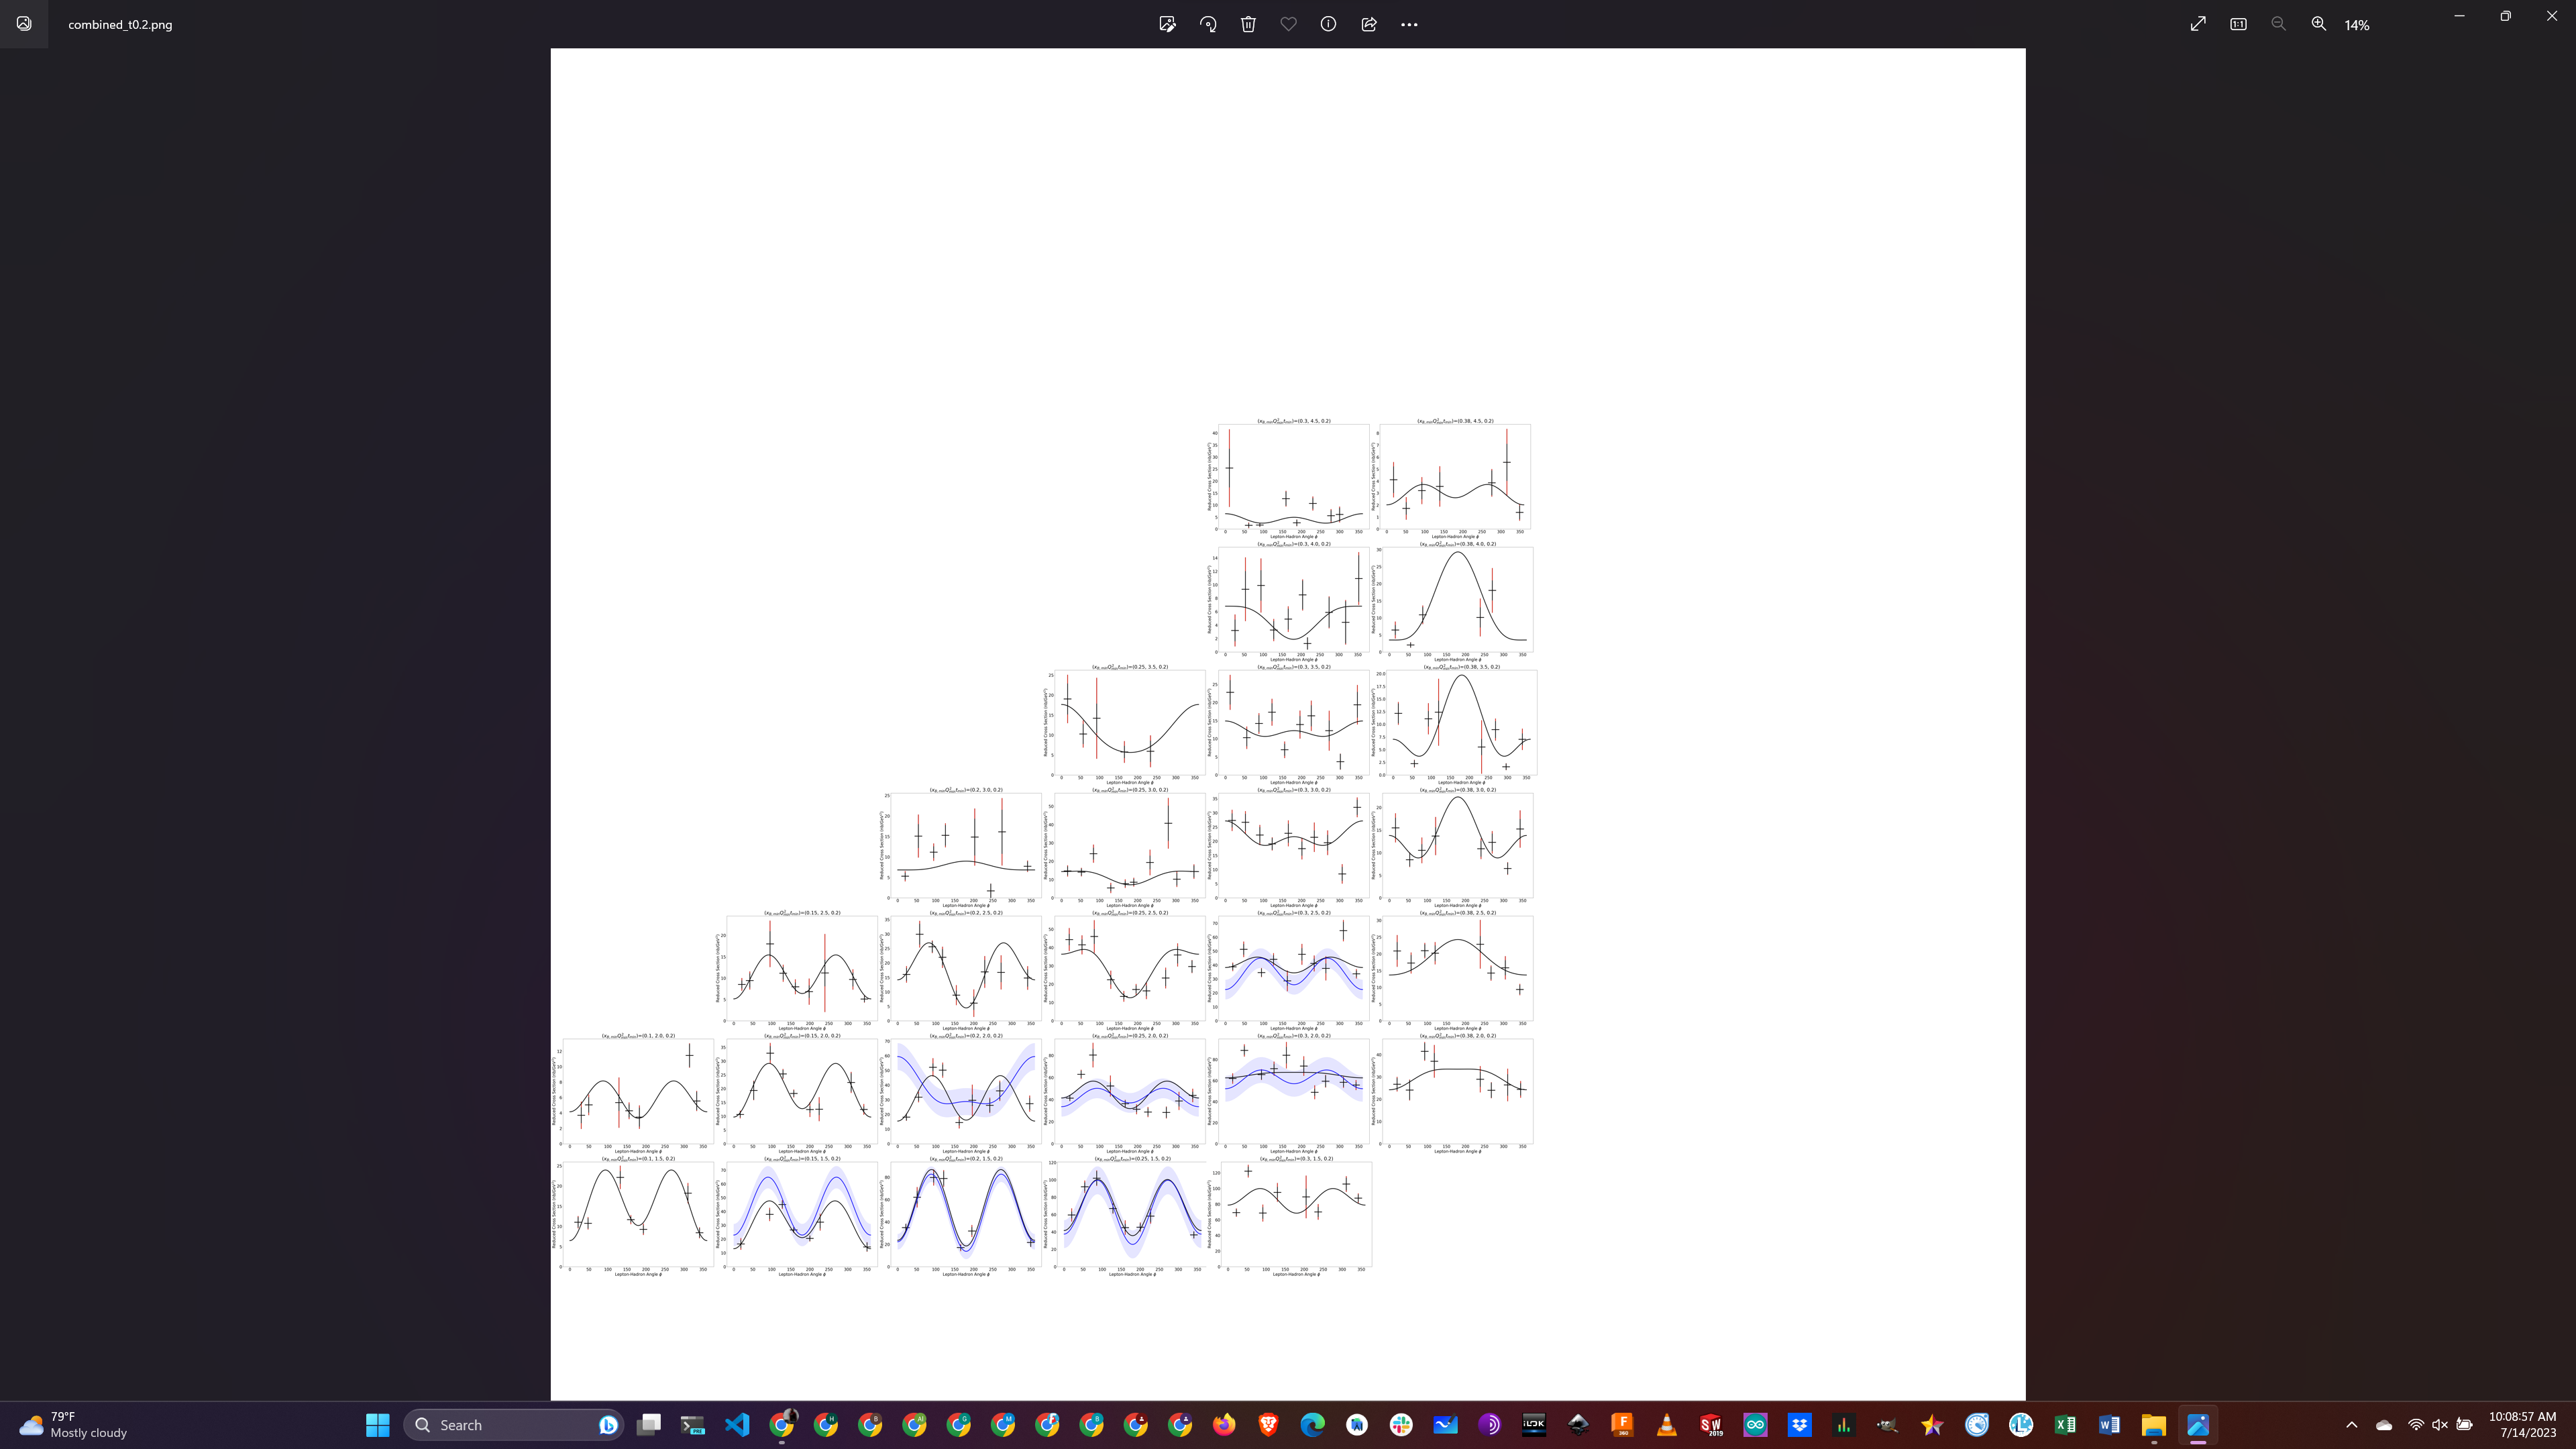
\includegraphics[trim={14.6cm 4cm 27.2cm 4cm},clip,width=\textwidth]{Chapters/Ch4-BaseAnalysis/bin_by_bin_cross_sections/pics_screenshots/t_2.png}
\caption[Reduced Cross Section for 0.2 $GeV^2 < t <$ 0.3 $ GeV^2$]{Reduced Cross Section for 0.2 $ GeV^2 < t <$ 0.3 $GeV^2$ in bins of $x_B$ (increasing left to right) and $Q^2$ (increasing vertically upwards). }
\label{fig:combined_t0.2}
\end{figure}


\begin{figure}[ht]
\centering
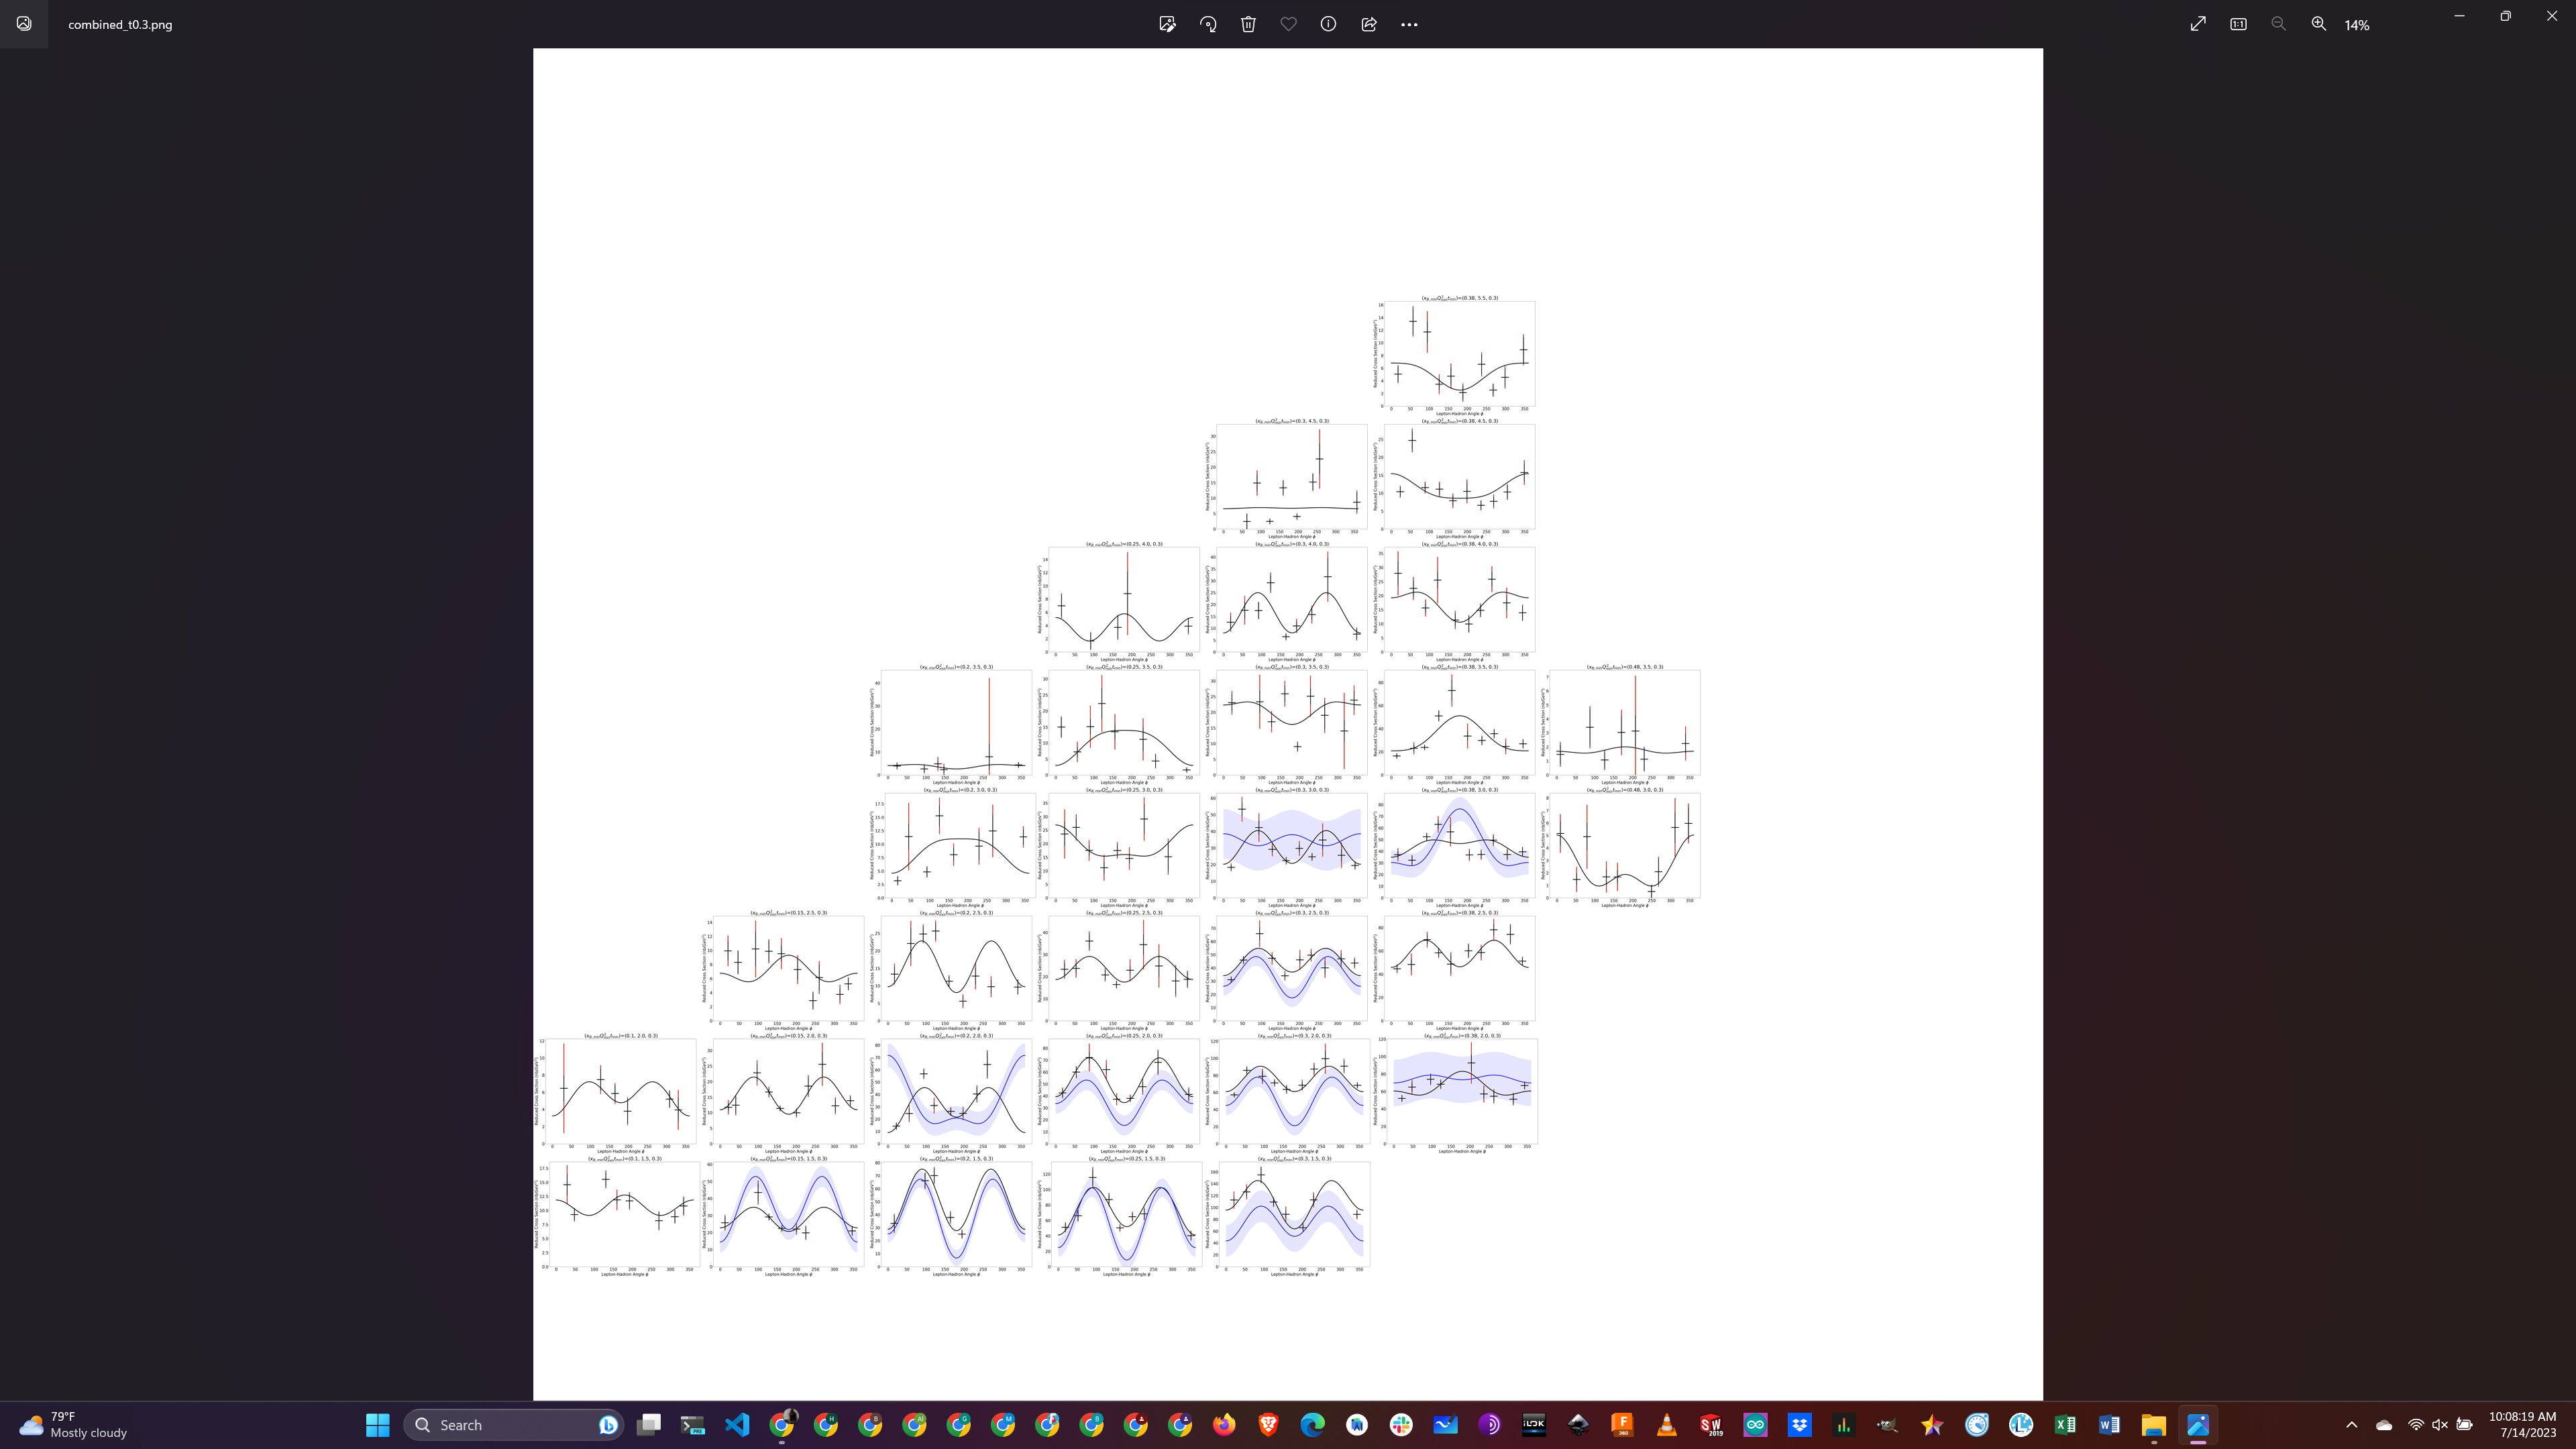
\includegraphics[trim={14.1cm 4cm 27.2cm 4cm},clip,width=\textwidth]{Chapters/Ch4-BaseAnalysis/bin_by_bin_cross_sections/pics_screenshots/t_3.png}
\caption[Reduced Cross Section for 0.3 $GeV^2 < t <$ 0.4 $ GeV^2$]{Reduced Cross Section for 0.3 $ GeV^2 < t <$ 0.4 $GeV^2$.}
\label{fig:combined_t0.3}
\end{figure}


\begin{figure}[ht]
\centering
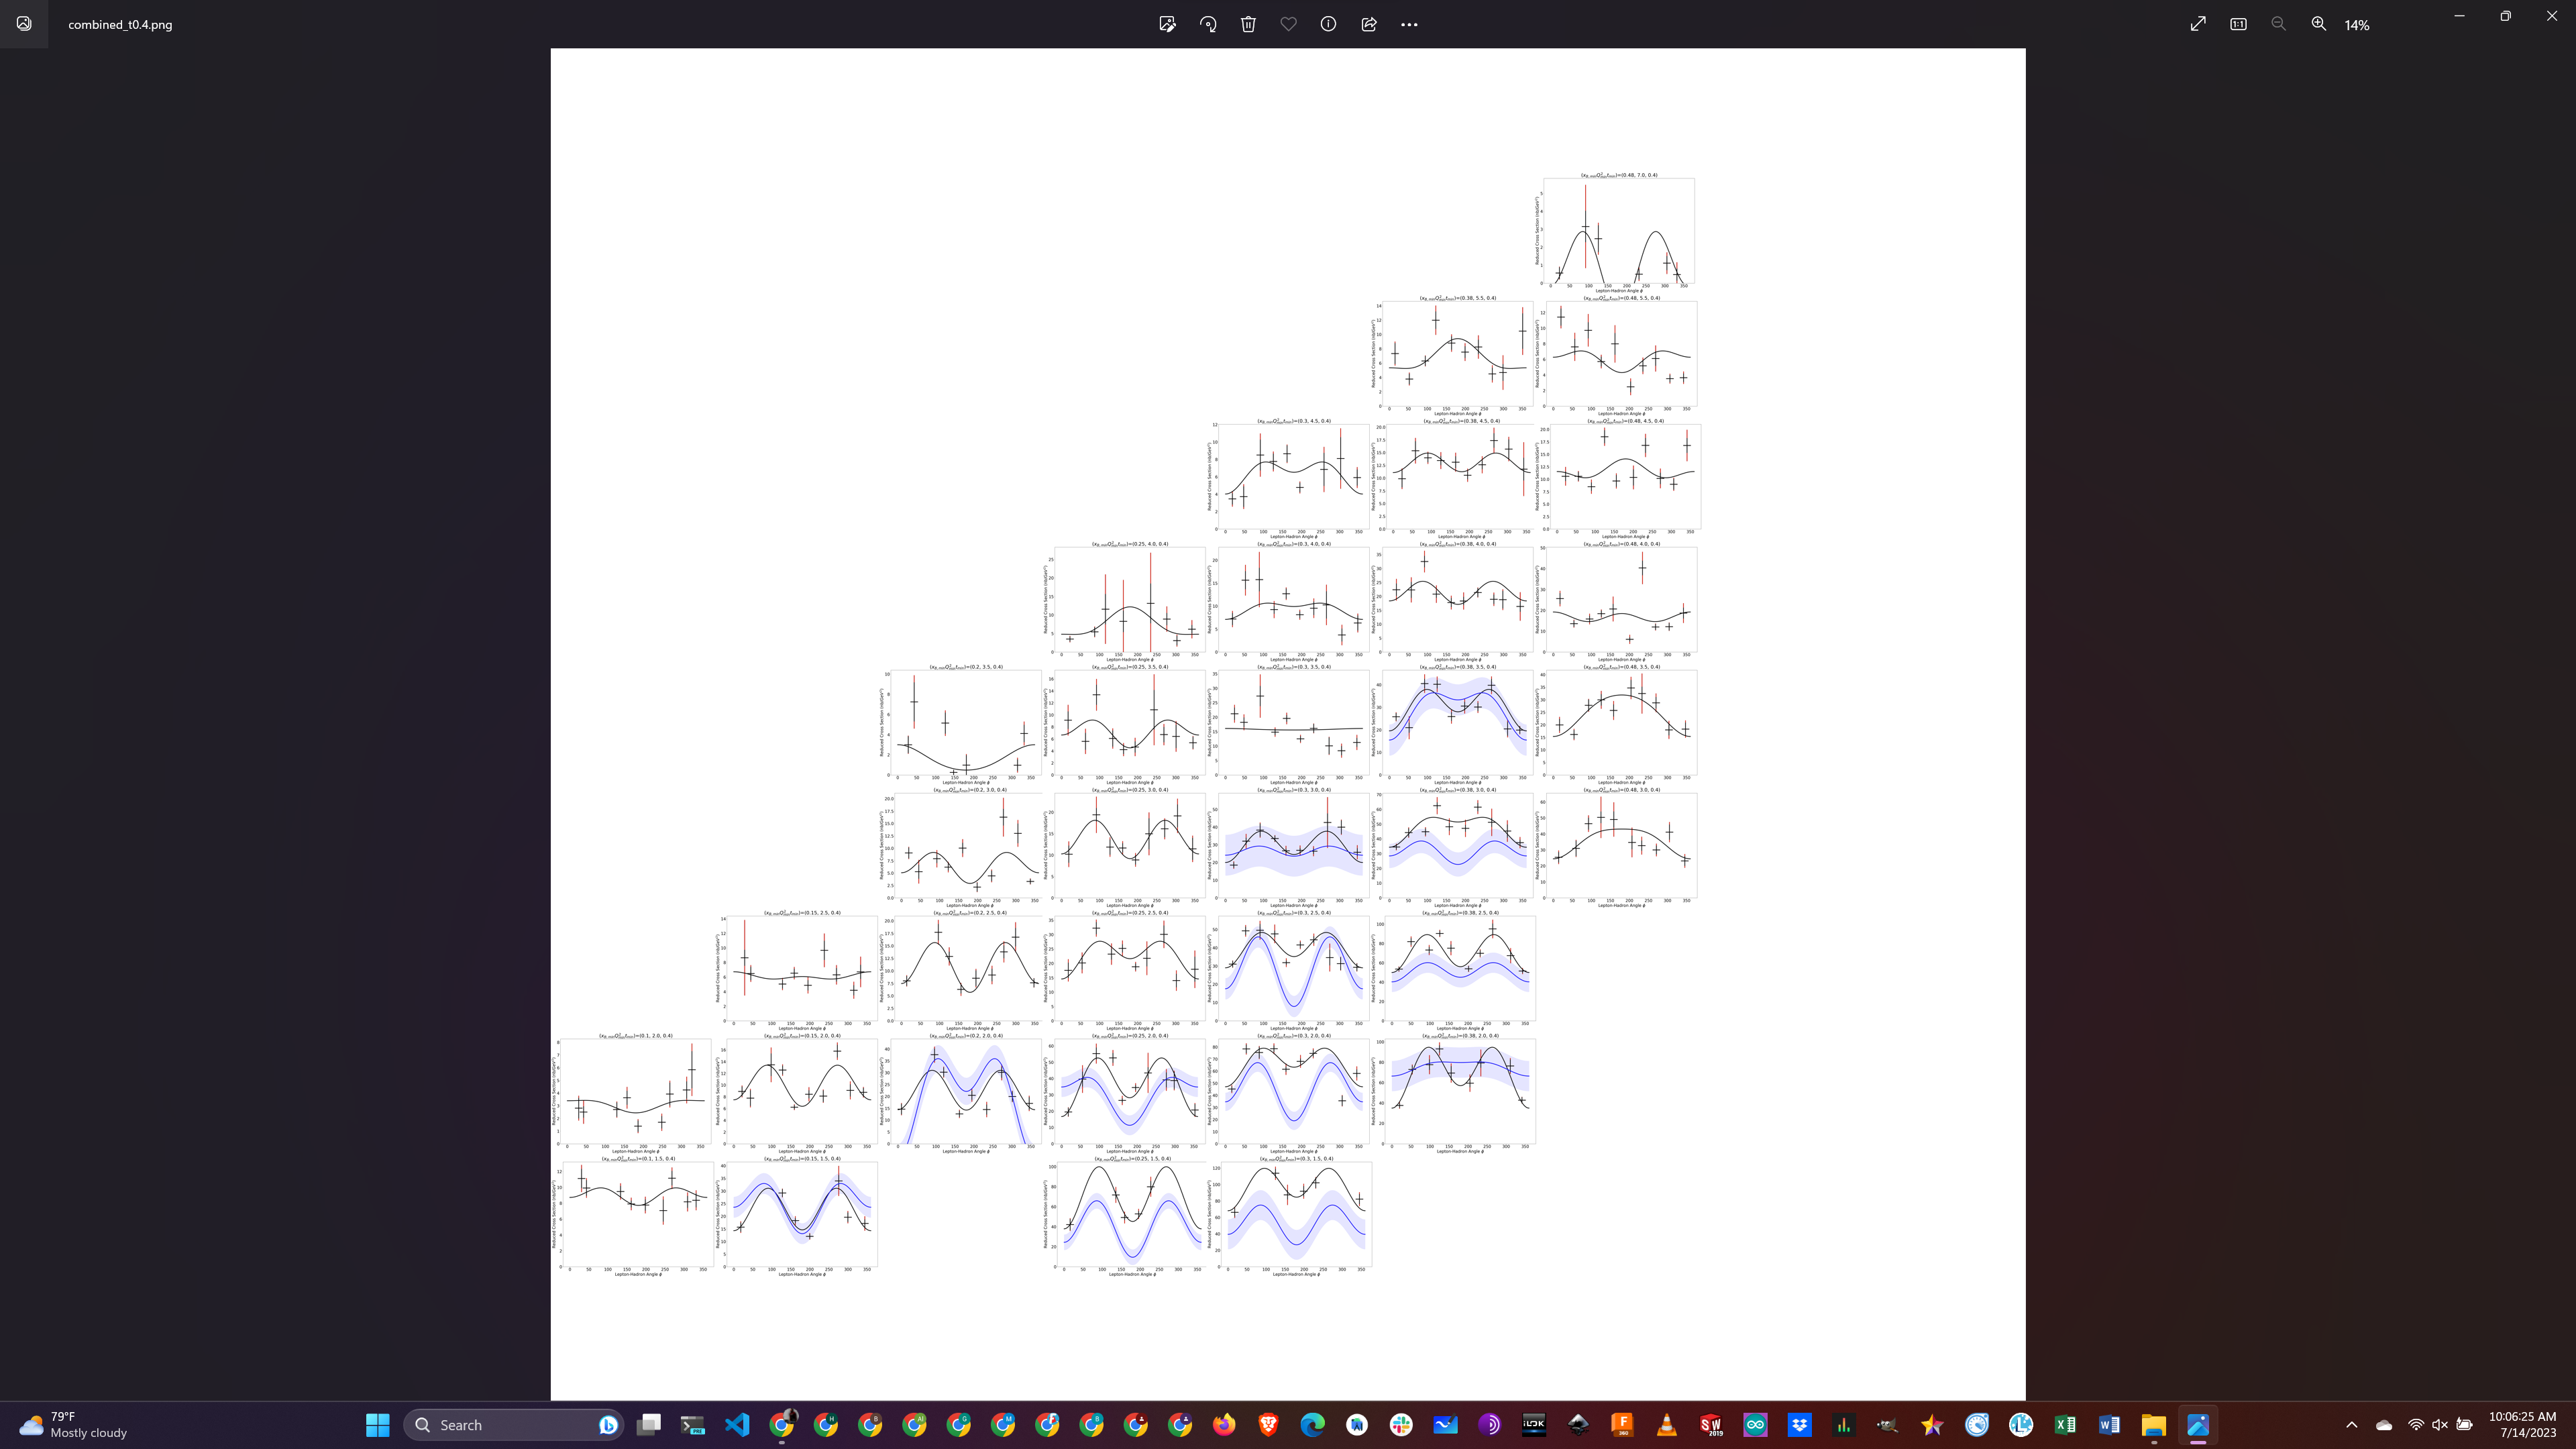
\includegraphics[trim={14.6cm 4cm 23cm 4cm},clip,width=\textwidth]{Chapters/Ch4-BaseAnalysis/bin_by_bin_cross_sections/pics_screenshots/t_4.png}
\caption[Reduced Cross Section for 0.4 $GeV^2 < t <$ 0.6 $GeV^2$]{Reduced Cross Section for 0.4 $GeV^2 < t <$ 0.6 $GeV^2$.}
\label{fig:combined_t0.4}
\end{figure}


\begin{figure}[ht]
    \centering
    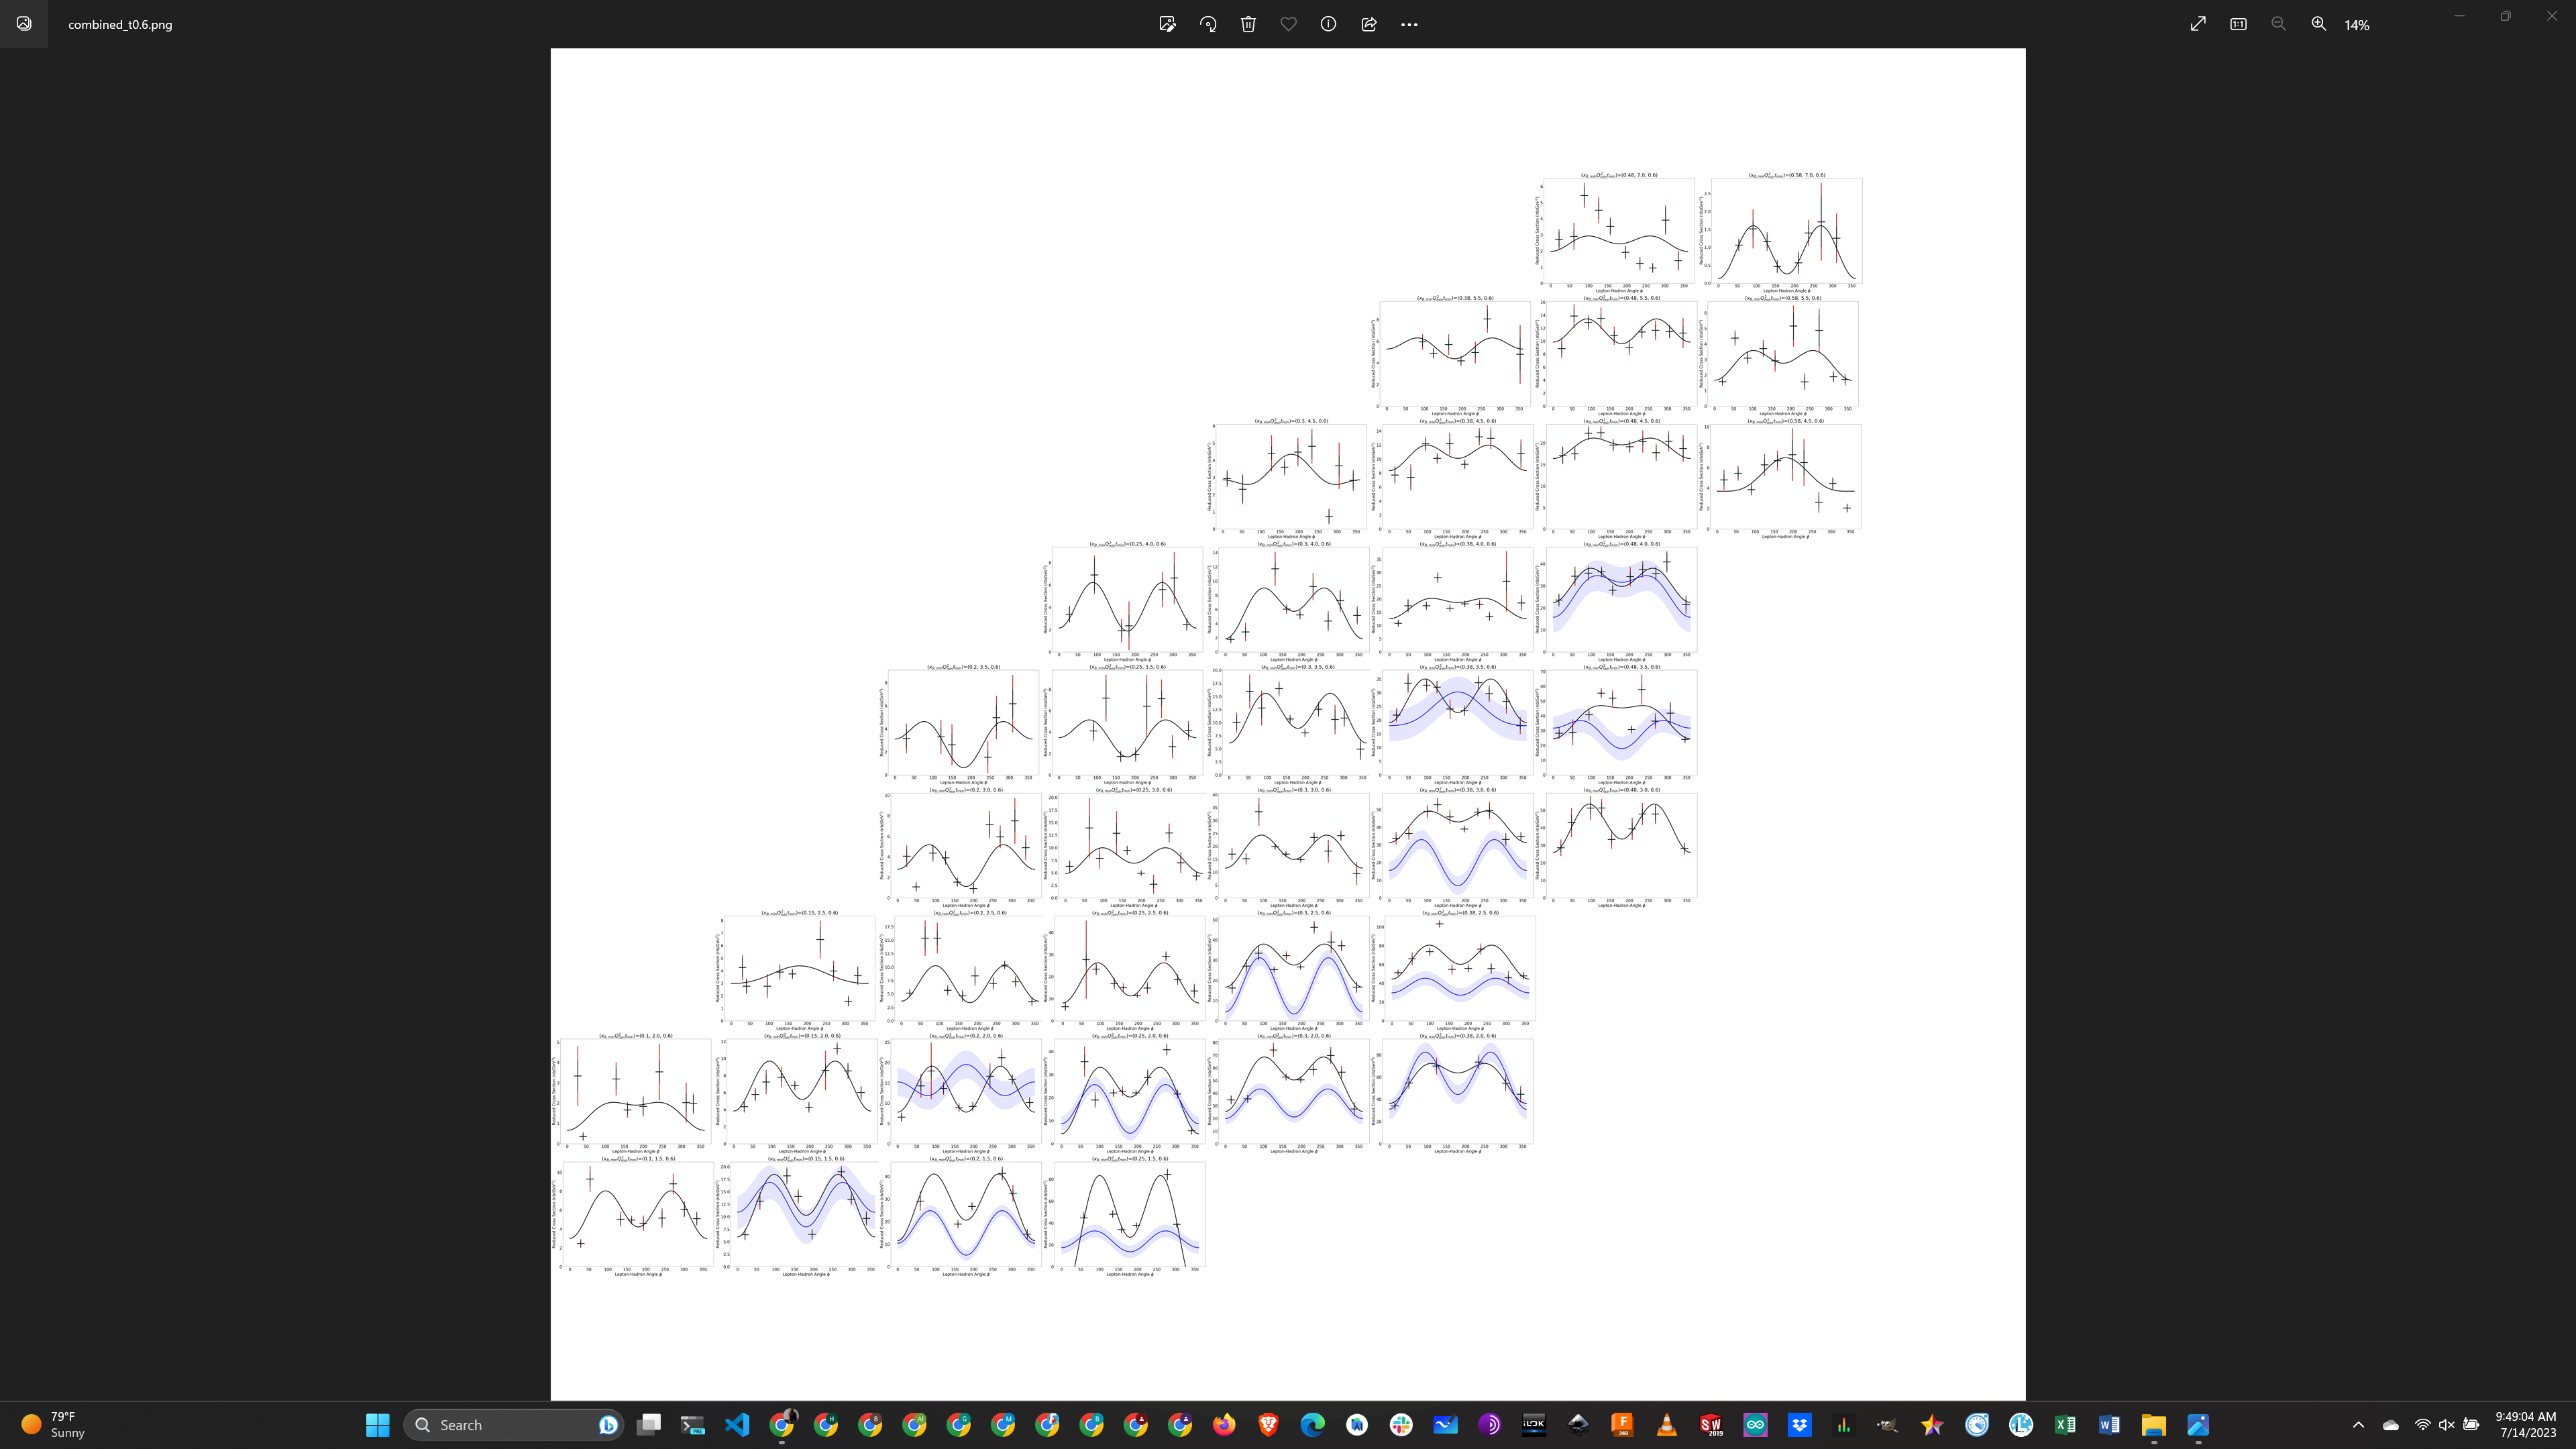
\includegraphics[trim={14.8cm 4cm 18.5cm 4cm},clip,width=\textwidth]{Chapters/Ch4-BaseAnalysis/bin_by_bin_cross_sections/pics_screenshots/t_6.png}
    \caption[Reduced Cross Section for 0.6 $GeV^2 < t <$ 1.0 $GeV^2$]{Reduced Cross Section for 0.6 $GeV^2 < t <$ 1.0 $GeV^2$.}
    \label{fig:combined_t0.6}
\end{figure}


\begin{figure}[ht]
    \centering
    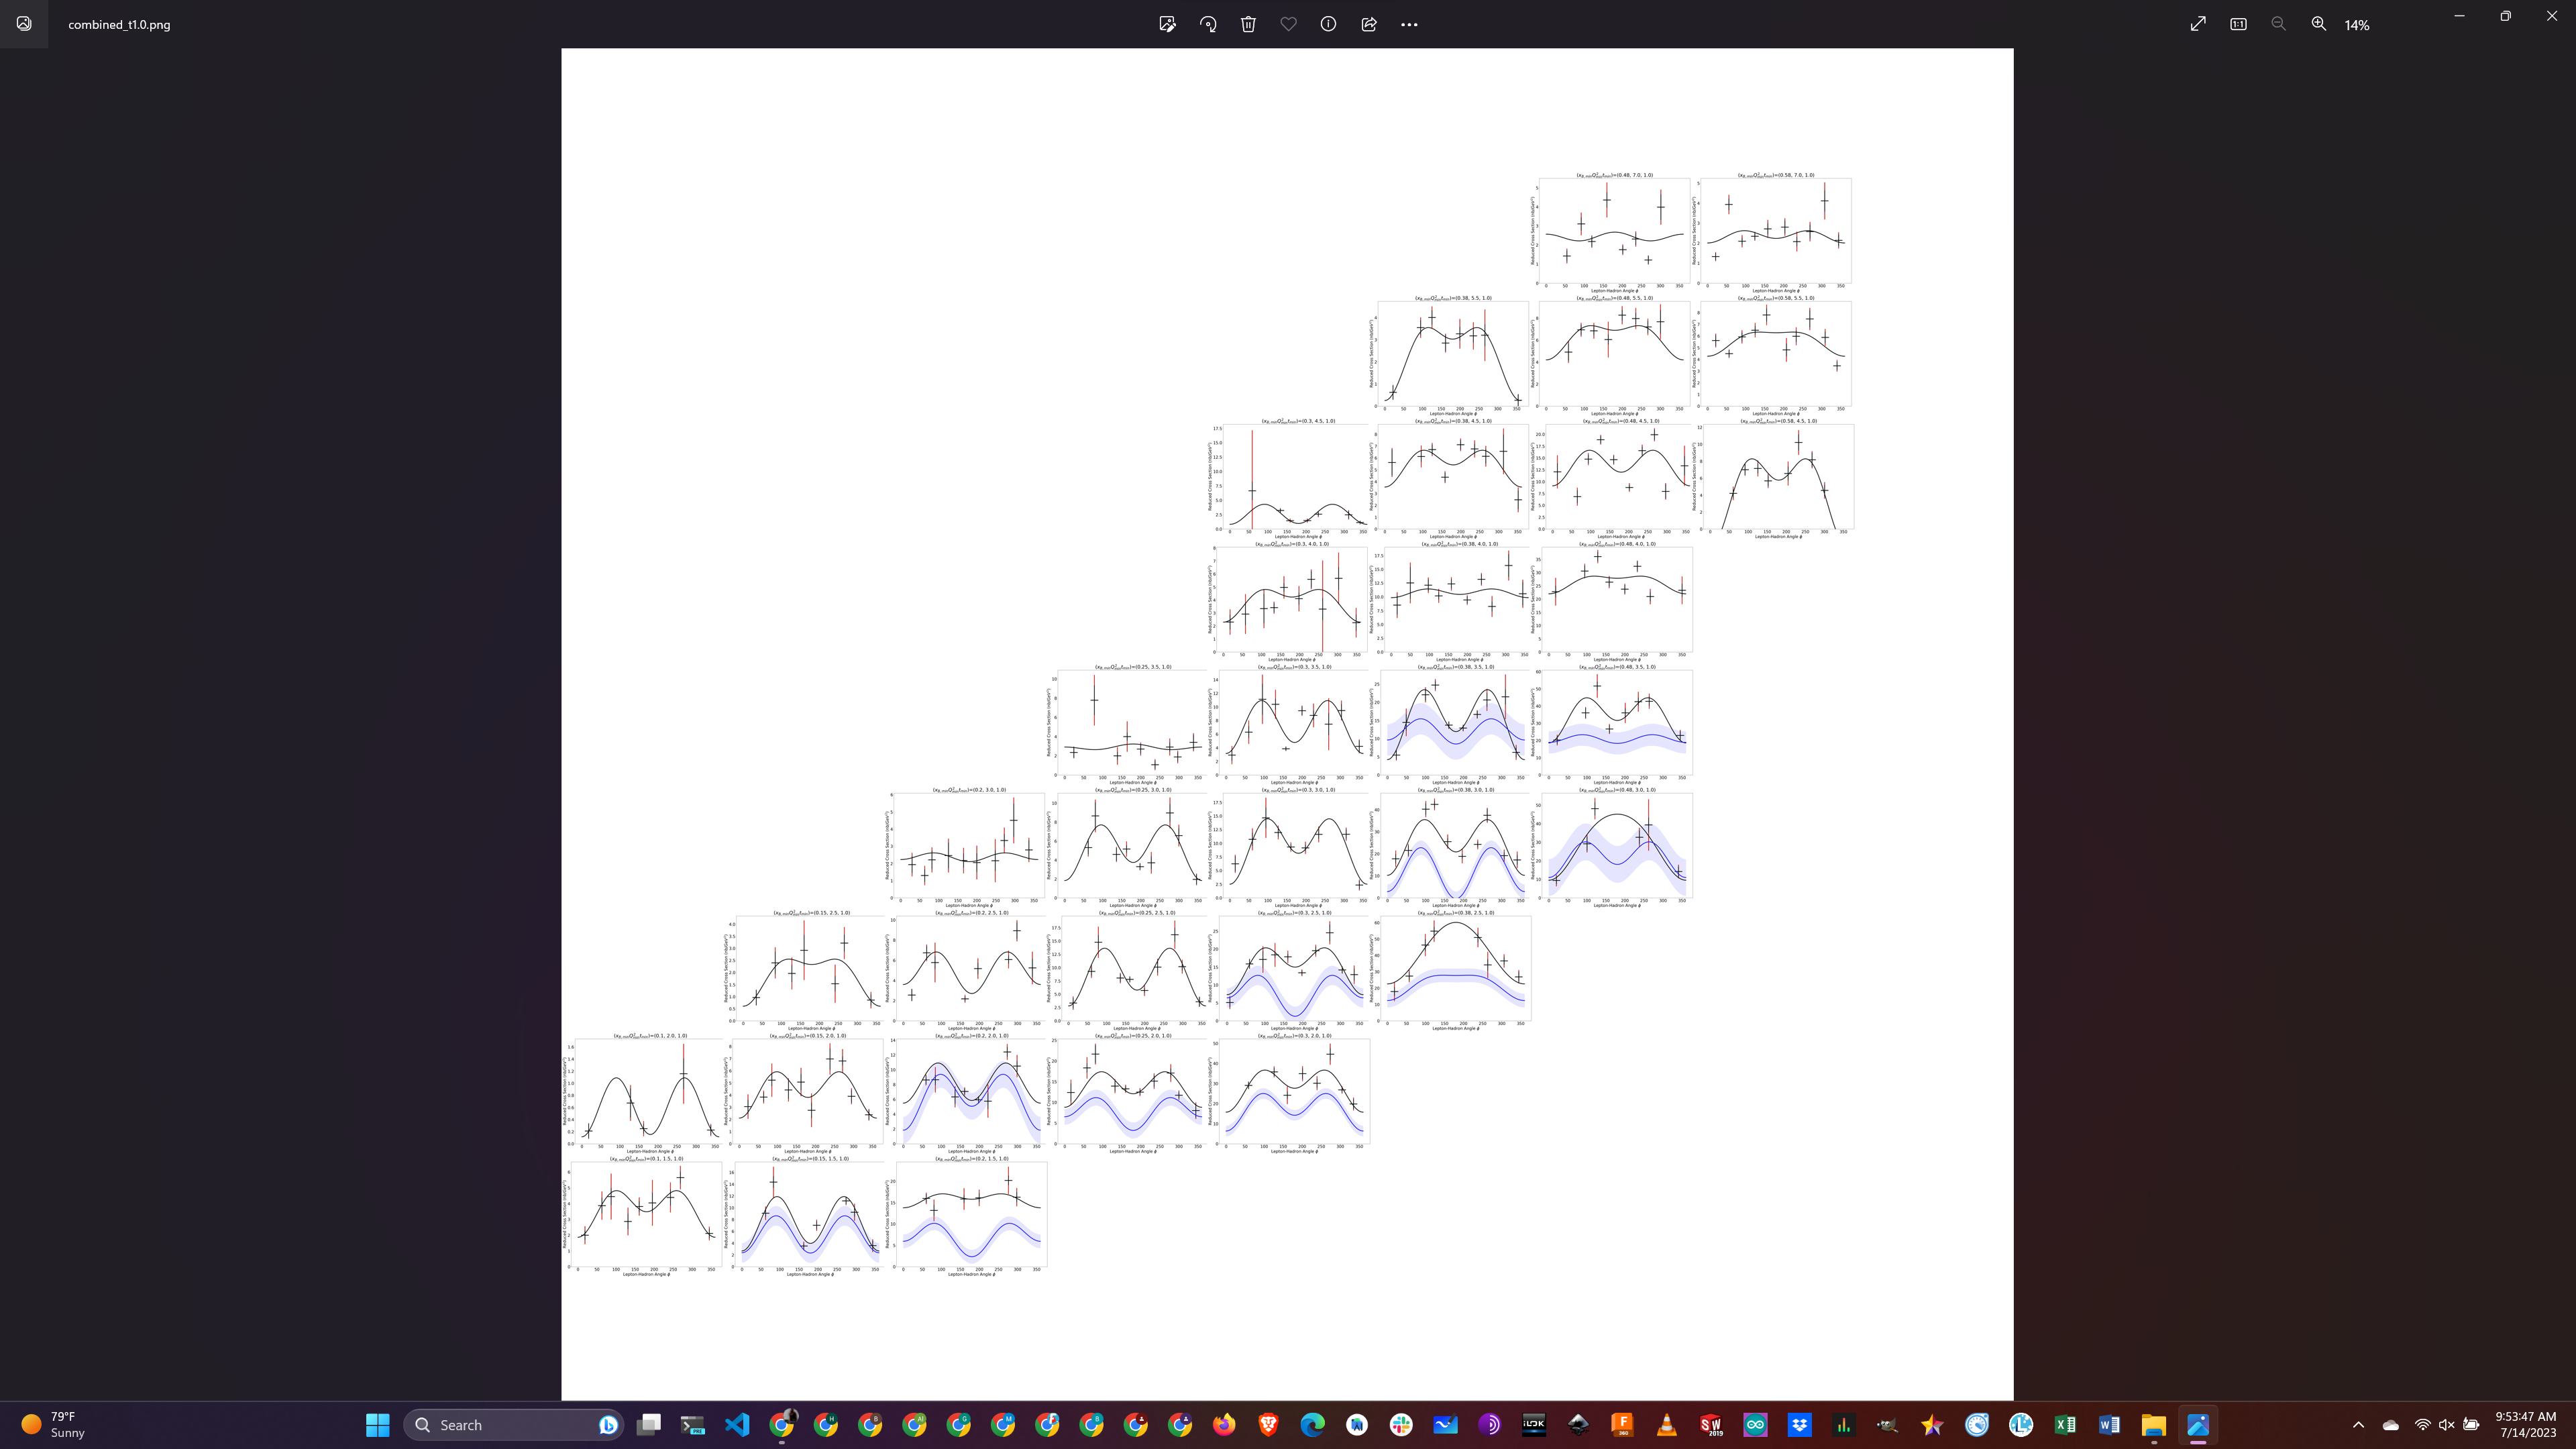
\includegraphics[trim={14.8cm 4cm 18.5cm 4cm},clip,width=\textwidth]{Chapters/Ch4-BaseAnalysis/bin_by_bin_cross_sections/pics_screenshots/t_10.png}
    \caption[Reduced Cross Section for 1.0 $GeV^2 < t <$ 1.5 $GeV^2$]{Reduced Cross Section for 1.0 $GeV^2 < t <$ 1.5 $GeV^2$.}
    \label{fig:combined_t1.0}
\end{figure}

\begin{figure}[ht]
    \centering
    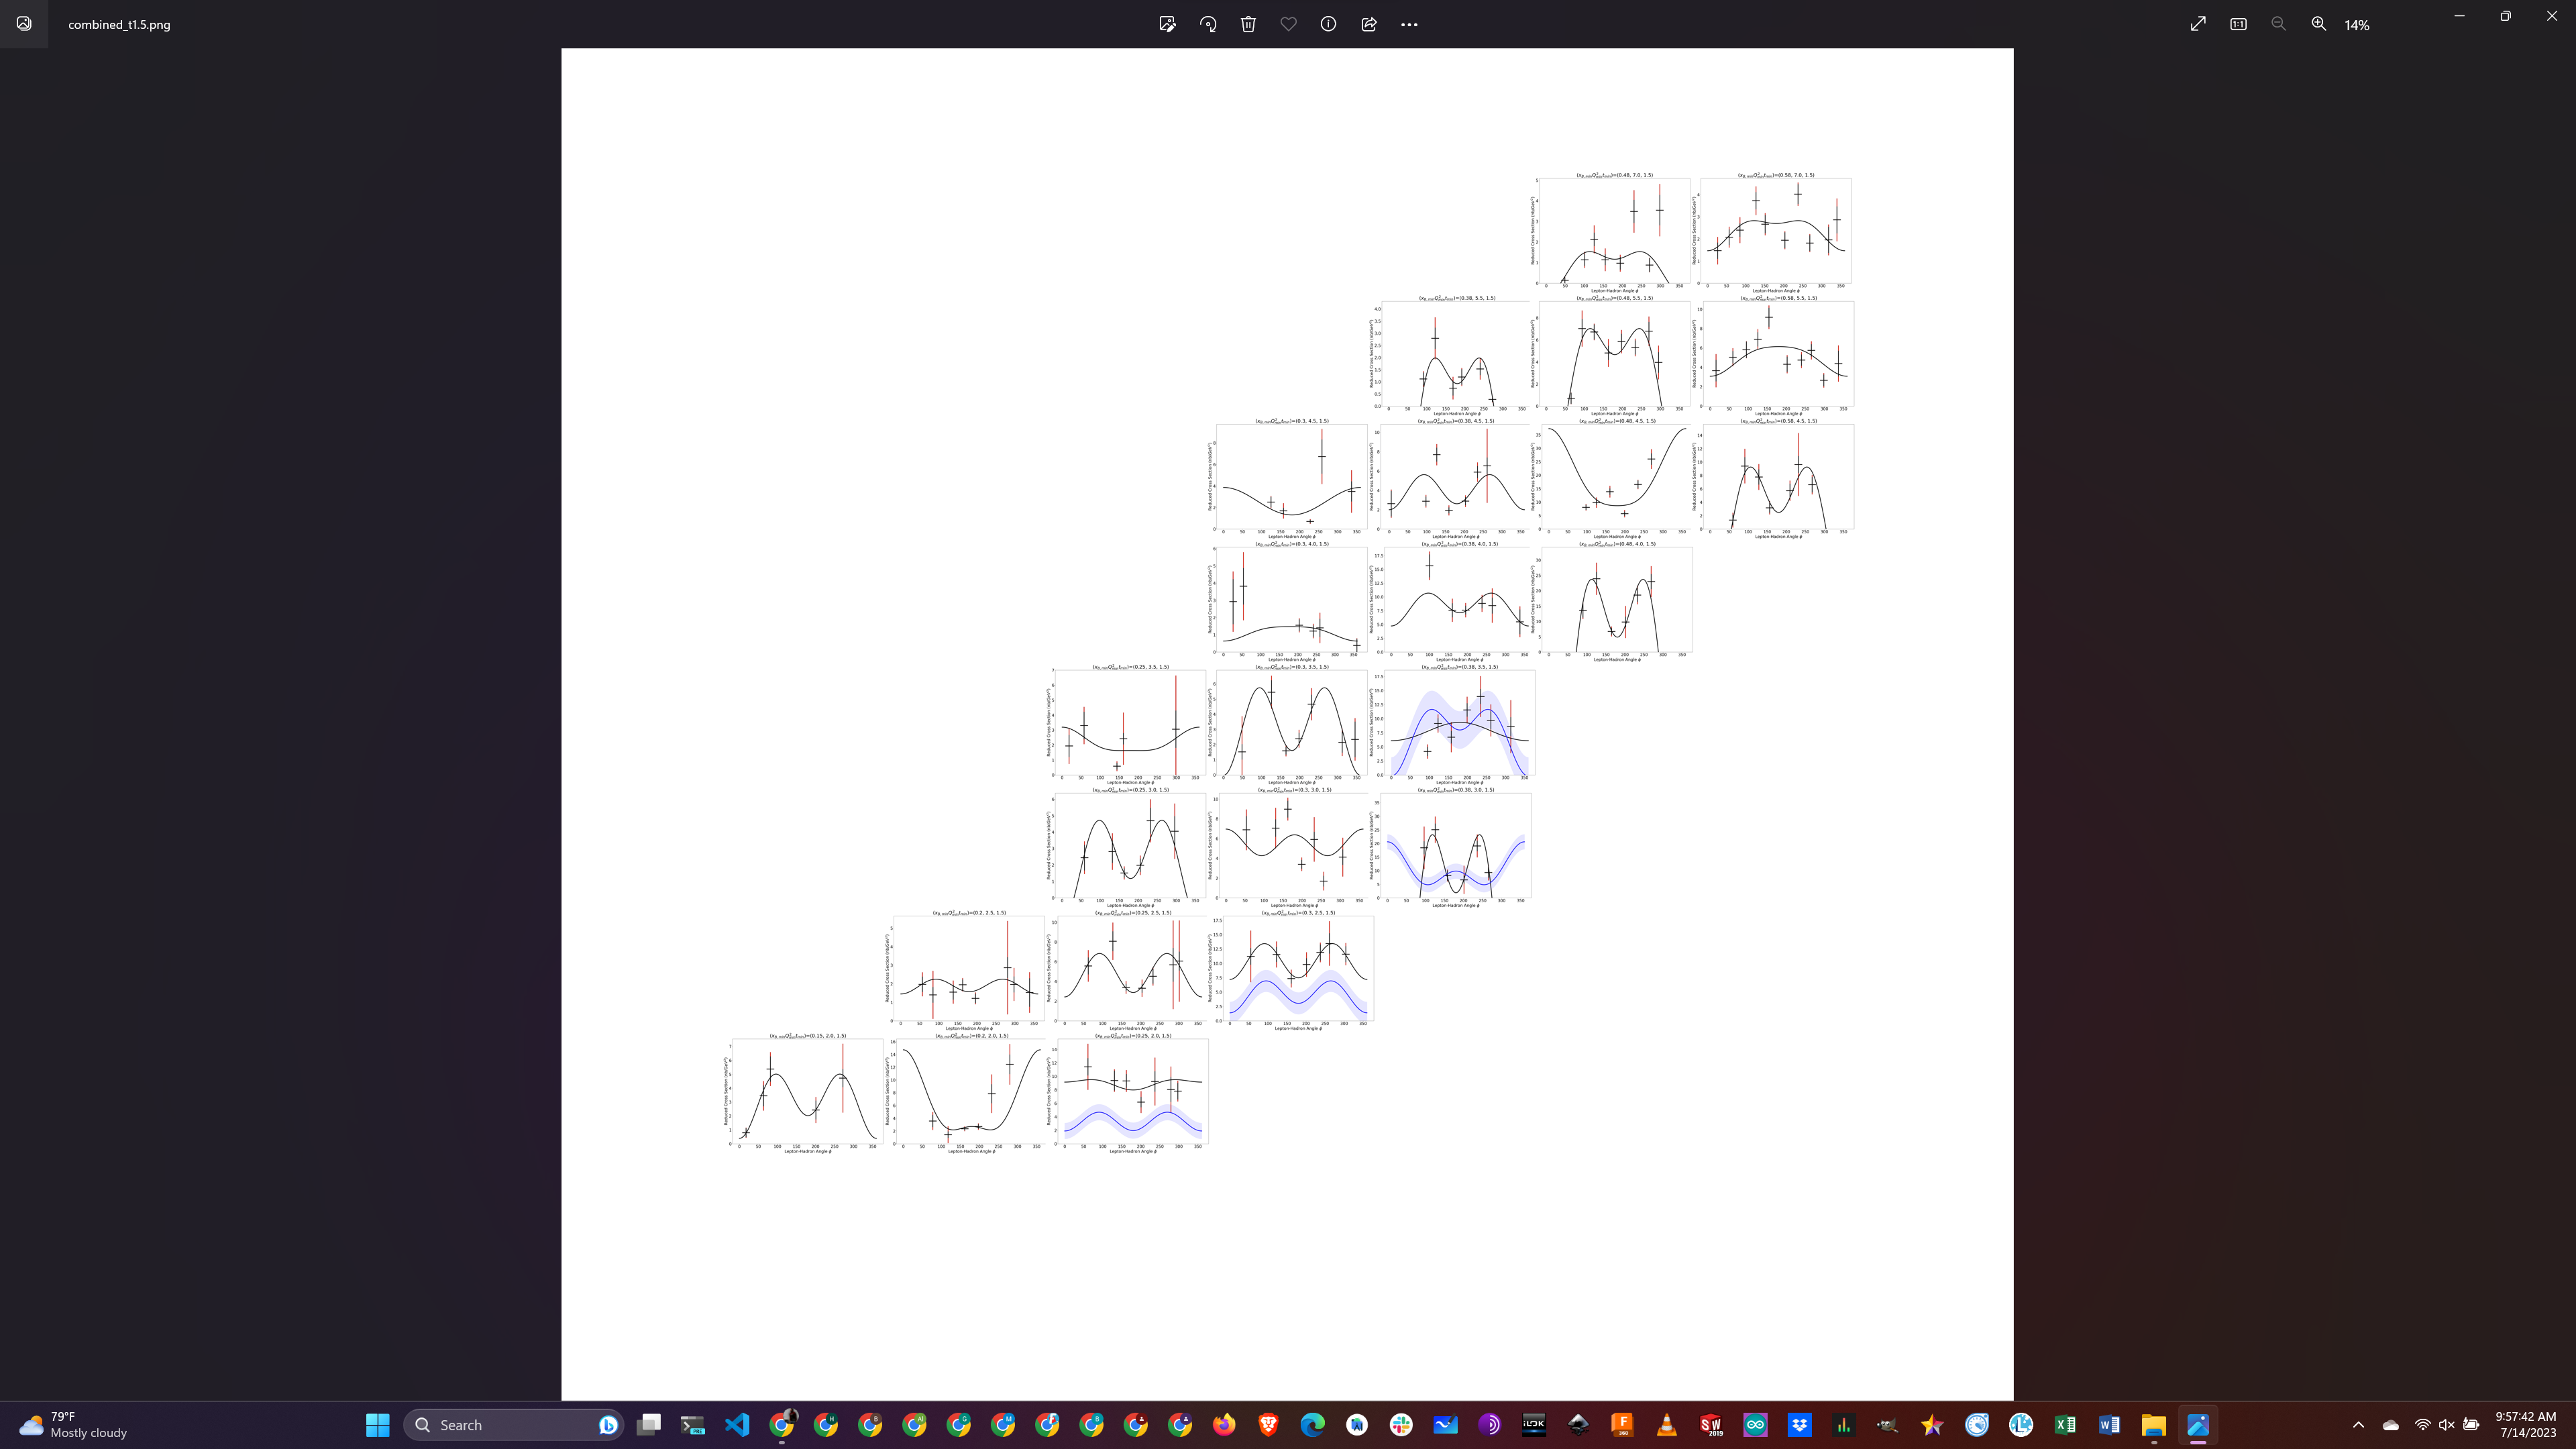
\includegraphics[trim={18.8cm 4cm 18.5cm 4cm},clip,width=\textwidth]{Chapters/Ch4-BaseAnalysis/bin_by_bin_cross_sections/pics_screenshots/t15.png}
    \caption[Reduced Cross Section for 1.5 $GeV^2 < t <$ 2.0 $GeV^2$]{Reduced Cross Section for 1.5 $GeV^2 < t <$ 2.0 $GeV^2$.}
    \label{fig:combined_t1.5}
\end{figure}

\fi